\subsection{UC3 - Visualizzazione 3D del magazzino}
\begin{figure}[H]
  \centering
  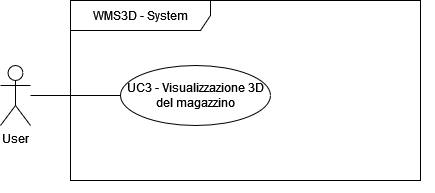
\includegraphics[width=0.8\textwidth]{UC_diagrams_1-10/UC3_sys.drawio.png}
   \caption{Diagramma UML UC3 - Visualizzazione 3D del magazzino}
\end{figure}
\begin{figure}[H]
  \centering
  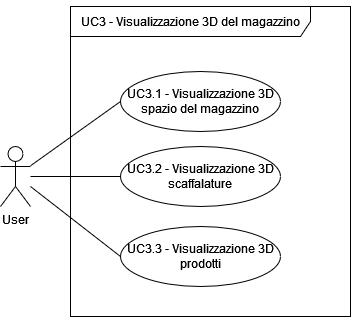
\includegraphics[width=0.5\textwidth]{UC_diagrams_1-10/UC3.drawio.png}
   \caption{Diagramma UML in dettaglio UC3 - Visualizzazione 3D del magazzino}
\end{figure}
\begin{itemize}
    \item \textbf{Attori:} User.
    \item \textbf{Pre-condizione:}  L'utente ha creato un magazzino [UC1].
    \item \textbf{Post-condizione:} L'utente può vedere il magazzino creato in 3D in tutte le sue parti.
    \item \textbf{Scenario Principale:}  L'utente visualizza interamente in 3D la planimetria del magazzino, in particolare può vedere lo spazio in sè del magazzino [UC3.1] e, se presenti, può visualizzare anche scaffalature [UC3.2] e prodotti [UC3.3].
    \item \textbf{Generalizzazioni:} -
    \item \textbf{Estensioni:} -
\end{itemize}


\subsubsection{UC3.1 - Visualizzazione 3D spazio del magazzino}
\begin{figure}[H]
  \centering
  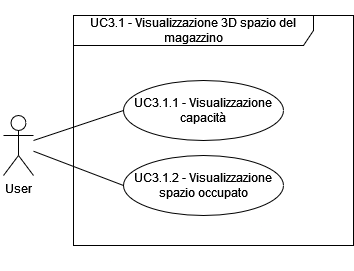
\includegraphics[width=0.6\textwidth]{UC_diagrams_1-10/UC3.1.drawio.png}
   \caption{Diagramma UML UC3.1 - Visualizzazione 3D spazio del magazzino}
\end{figure}
\begin{itemize}
    \item \textbf{Attori:} User.
    \item \textbf{Pre-condizione:} L'utente ha creato un magazzino [UC1].
    \item \textbf{Post-condizione:} L'utente visualizza in 3D lo spazio del magazzino.
    \item \textbf{Scenario Principale:}  L'utente può vederne in 3D lo spazio del magazzino, in particolare può notarne graficamente e in proporzione capacità del magazzino [UC3.1.1] e spazio occupato al suo interno [UC3.1.2].
    \item \textbf{Generalizzazioni:} -
    \item \textbf{Estensioni:} -
\end{itemize}


\paragraph{UC3.1.1 - Visualizzazione capacità}
\begin{itemize}
    \item \textbf{Attori:} User.
    \item \textbf{Pre-condizione:} L'utente ha creato un magazzino [UC1] e ne sta guardando lo spazio.
    \item \textbf{Post-condizione:} L'utente visualizza la capacità del magazzino.
    \item \textbf{Scenario Principale:}  L'utente, guardando allo spazio del magazzino creato dal render 3D, può notare la capacità (i.e. la grandezza) del magazzino.
    \item \textbf{Generalizzazioni:} -
    \item \textbf{Estensioni:} -
\end{itemize}


\paragraph{UC3.1.2 - Visualizzazione spazio occupato}
\begin{itemize}
    \item \textbf{Attori:} User.
    \item \textbf{Pre-condizione:} L'utente ha creato un magazzino [UC1] e ne sta guardando lo spazio.
    \item \textbf{Post-condizione:} L'utente visualizza lo spazio occupato all'interno del magazzino.
    \item \textbf{Scenario Principale:}  L'utente, guardando allo spazio del magazzino creato dal render 3D, può notare lo spazio occupato (i.e. la proporzione tra parti in cui sono posizionate scaffalature e parti vuote).
    \item \textbf{Generalizzazioni:} -
    \item \textbf{Estensioni:} -
\end{itemize}


\subsubsection{UC3.2 - Visualizzazione 3D scaffalature}
\begin{figure}[H]
  \centering
  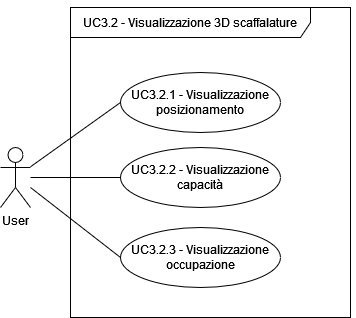
\includegraphics[width=0.6\textwidth]{UC_diagrams_1-10/UC3.2.drawio.png}
   \caption{Diagramma UML UC3.2 - Visualizzazione 3D scaffalature}
\end{figure}
\begin{itemize}
    \item \textbf{Attori:} User.
    \item \textbf{Pre-condizione:} L'utente ha creato un magazzino [UC1] al cui interno sono presenti delle scaffalature.
    \item \textbf{Post-condizione:} L'utente visualizza in 3D le scaffalature all'interno del magazzino.
    \item \textbf{Scenario Principale:}  L'utente può vedere in 3D le scaffalature all'interno del magazzino, in particolare potrà notarne (graficamente) il posizionamento [UC3.2.1], la capacità [UC3.2.2] e lo spazio occupato al suo interno [UC3.2.3].
    \item \textbf{Generalizzazioni:} -
    \item \textbf{Estensioni:} -
\end{itemize}


\paragraph{UC3.2.1 - Visualizzazione posizionamento}
\begin{itemize}
    \item \textbf{Attori:} User.
    \item \textbf{Pre-condizione:} L'utente ha creato un magazzino [UC1] al cui interno sono presenti delle scaffalature a cui l'utente sta guardando.
    \item \textbf{Post-condizione:} L'utente visualizza il posizionamento delle scaffalature all'interno del magazzino.
    \item \textbf{Scenario Principale:} L'utente, guardando alle scaffalature presenti nel magazzino dal render 3D, può notarne la loro posizione e disposizione all'interno del magazzino.
    \item \textbf{Generalizzazioni:} -
    \item \textbf{Estensioni:} -
\end{itemize}


\paragraph{UC3.2.2 - Visualizzazione capacità}
\begin{itemize}
    \item \textbf{Attori:} User.
    \item \textbf{Pre-condizione:} L'utente ha creato un magazzino [UC1] al cui interno sono presenti delle scaffalature a cui l'utente sta guardando.
    \item \textbf{Post-condizione:} L'utente visualizza la capacità delle scaffalature all'interno dell magazzino.
    \item \textbf{Scenario Principale:}  L'utente, guardando alle scaffalature presenti nel magazzino dal render 3D, può notarne la loro capacità, ovvero il numero di bin\textsuperscript{G} da cui sono composte.
    \item \textbf{Generalizzazioni:} -
    \item \textbf{Estensioni:} -
\end{itemize}


\paragraph{UC3.2.3 - Visualizzazione occupazione}
\begin{itemize}
    \item \textbf{Attori:} User.
    \item \textbf{Pre-condizione:} L'utente ha creato un magazzino [UC1] al cui interno sono presenti delle scaffalature a cui l'utente sta guardando.
    \item \textbf{Post-condizione:} L'utente visualizza lo stato di occupazione delle scaffalature all'interno del magazzino.
    \item \textbf{Scenario Principale:}  L'utente, guardando alle scaffalature presenti nel magazzino dal render 3D, può notarne la loro occupazione (i.e. la proporzione tra parti in cui sono posizionati prodotti e le parti libere).
    \item \textbf{Generalizzazioni:} -
    \item \textbf{Estensioni:} -
\end{itemize}


\subsubsection{UC3.3 - Visualizzazione 3D prodotti}
\begin{figure}[H]
  \centering
  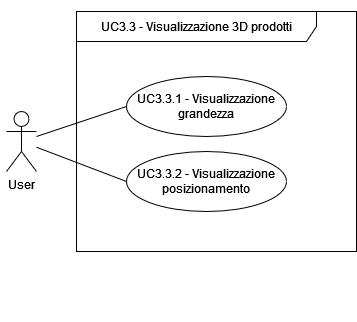
\includegraphics[width=0.6\textwidth]{UC_diagrams_1-10/UC3.3.drawio.png}
   \caption{Diagramma UML UC3.3 - Visualizzazione 3D prodotti}
\end{figure}
\begin{itemize}
    \item \textbf{Attori:} User.
    \item \textbf{Pre-condizione:}  L'utente ha creato un magazzino [UC1] al cui interno sono presenti delle scaffalature e dei prodotti posizionati.
    \item \textbf{Post-condizione:} L'utente visualizza in 3D i prodotti posizionati nelle scaffalature all'interno del magazzino.
    \item \textbf{Scenario Principale:}  L'utente può vedere in 3D i prodotti posizionati sulle scaffalature all'interno del magazzino, in particolare potrà notarne (graficamente) la grandezza [UC3.3.1] e il posizionamento [UC3.3.2].
    \item \textbf{Generalizzazioni:} -
    \item \textbf{Estensioni:} -
\end{itemize}


\paragraph{UC3.3.1 - Visualizzazione grandezza}
\begin{itemize}
    \item \textbf{Attori:} User.
    \item \textbf{Pre-condizione:} L'utente ha creato un magazzino [UC1] al cui interno sono presenti delle scaffalature e dei prodotti posizionati. L'utente sua guardando questi ultimi.
    \item \textbf{Post-condizione:} L'utente visualizza la grandezza dei prodotti posizionati nelle scaffalature all'interno del magazzino.
    \item \textbf{Scenario Principale:} L'utente, guardando ai prodotti presenti nel magazzino dal render 3D, può notarne la loro dimensione.
    \item \textbf{Generalizzazioni:} -
    \item \textbf{Estensioni:} -
\end{itemize}


\paragraph{UC3.3.2 - Visualizzazione posizionamento}
\begin{itemize}
    \item \textbf{Attori:} User.
    \item \textbf{Pre-condizione:} L'utente ha creato un magazzino [UC1] al cui interno sono presenti delle scaffalature e dei prodotti posizionati. L'utente sua guardando questi ultimi.
    \item \textbf{Post-condizione:} L'utente visualizza in quali scaffalature sono posizionati i prodotti all'interno del magazzino.
    \item \textbf{Scenario Principale:}  L'utente, guardando ai prodotti presenti nel magazzino dal render 3D, può notarne il loro posizionamento e disposizione (i.e. in quale scaffalatura e in quale bin\textsuperscript{G} i prodotti sono posizionati).
    \item \textbf{Generalizzazioni:} -
    \item \textbf{Estensioni:} -
\end{itemize}